\documentclass[report]{../../custom}
\begin{document}
\maketitle

\section{Coding reading}

On the last weekly, we had to read the paper and do some coding, we had figured out the SPHINCS+ all the compent, we will use the SPX to repalce the SPHINCS+, for the SPX, it have the three compent.

on the top level see, the SPX have the arithy length mssage $msg$ for it inupt, then on the signer have it own sercurity key $sk_{seed}$, and public key $pk_{seed}$. So the auth message, it like $SPX_{sign}: (msg,sk_{seed}) \mapsto (pk_{root},auth)$. then we will by the detial to saw the signature proposs.

first the $msg$ to the hash function, i.e. which function can chose differen sercurity level, by the hash fucntion it will out put the one have value $hm$, $tree_{index}$, for the FORS sign and HT sign (muti XMSS tree) respectily.

\subsection{FOTS}
then we have the $n$ bytes lenght of the $hm$, this is the hash function output the fix value, for the specific verison SPX. So we will do the FORS singture,
first spilt the $8\times n$ bit $hm$ dividel by the FORS tree height $t$, where the tree leaf node number is $2^t$. here $t | (8\times n)$. the $k\times t=(8\times n)$, the $k$ is the number of FORS tree. on the FORS leaf node is the random creat the $sk$ by the $sk_{seed}$ and other field.
all the leaf node by the $sk_{1\dots k}$ by the hash function for the low height level node, then the $k$ tree will split to compute the different root node. finally use the all the root node hash to the $FORS_{pk}$. on the FORS the $auth$, is the aside the node by the $hm$ spilt to $k$ index.
we use the figure~\ref{fig:fors_tree} to show the FORS auth node and pulic node by the red color node, the green color node need the $pk$ to computer by the verifier, based on the hashchian to do the one way function, we talked on the WOTS+ signtures.

\begin{figure}[h!]
	\begin{center}
		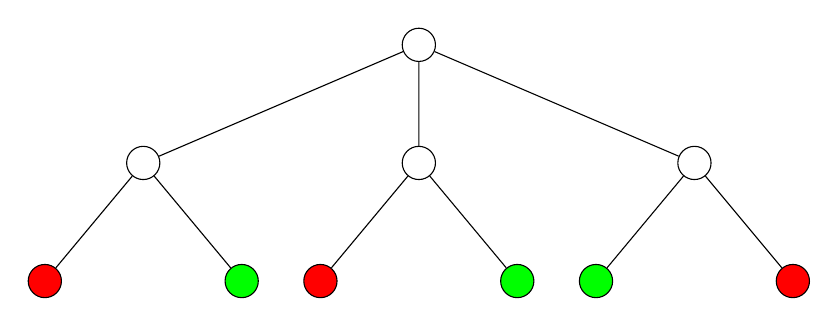
\begin{tikzpicture}[level distance=1.5cm,
				level 1/.style={sibling distance=3.5cm},
				level 2/.style={sibling distance=2.5cm},
				every node/.style={circle, draw, fill=white, inner sep=4pt, minimum size=12pt}]
			% Root node
			\node (root) [] {}
			% First level
			child {node [] {}
					% Second level
					child {node [fill=red!100] {}}
					child {node [fill=green!100] {}}
				}
			child {node [] {}
					% Second level
					child {node [fill=red!100] {}}
					child {node [fill=green!100] {}}
				}
			child {node [] {}
					% Second level
					child {node [fill=green!100] {}}
					child {node [fill=red!100] {}}
				};

		\end{tikzpicture}

	\end{center}
	\caption{The example FORS tree, here the $k=3,t=1$. the red node show the public info, the green node need use the $pk$ to computer.}\label{fig:fors_tree}
\end{figure}

\subsection{HT tree}

so by the we have the $n$ byte FOTS tree root, for the HT start computer node, on the FORS the $t$ is the markle tree height, on the HT tree the $h'$ is the number height - 1, respective the auth path need node. different the $k$ makle tree to concation, the HT tree have $d$ layer makle tree to computer the fianl public root node, which is the final public node.
on the Figure~\ref{fig:HT_tree}, the red is the auth path node and final public node by the red color highlight, the green node is by the WOTS+ signature, based on the hashchain. here use the fix lenght hashchain the start node is creat by the $sk_{seed}$, the $w$ step the chain will be the leaf node of XMSS tree.


\begin{figure}[htp!]
	\begin{center}
		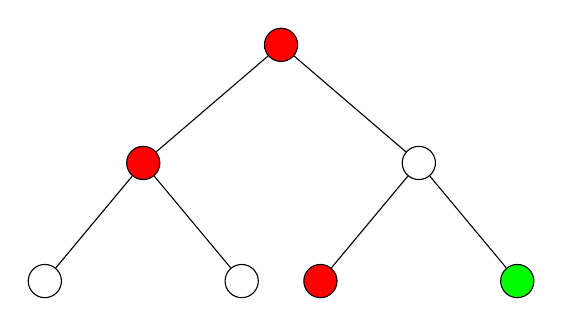
\begin{tikzpicture}[level distance=1.5cm,
				level 1/.style={sibling distance=3.5cm},
				level 2/.style={sibling distance=2.5cm},
				every node/.style={circle, draw, fill=white, inner sep=4pt, minimum size=12pt}]
			% Root node
			\node (root) [fill=red!100] {}
			% First level
			child {node [fill=red!100] {}
					% Second level
					child {node [] {}}
					child {node [] {}}
				}
			child {node [] {}
					% Second level
					child {node [fill=red!100] {}}
					child {node [fill=green!100] {}}
				};

		\end{tikzpicture}

	\end{center}
	\caption{The example HT tree, here the $h'=1,d=2$. the red node show the public info, the green node need use the FORS root node to computer by the hashchain.}\label{fig:HT_tree}
\end{figure}

The HT leaf node need the WOTS+ signature to computer, this is the HT computer start point. The Figure~\ref{fig:hashchain} show the hash chain use by the WOTS+ fignature, on the chian the blue color node is the private node creat by the $sk_{seed}$, there chain lenght $w=2$, so by the $FORS_{sign}$ it one bit is map to the red color node value for public, on the verify phase, let the red nood go to computer the step, then get the green node. which is the XMSS tree leaf node, add the Figure~\ref{fig:HT_tree} red auth node, we can caclute the HT root node. finish the signture.

\begin{figure}
	\begin{center}
		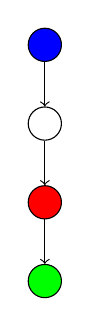
\begin{tikzpicture}[level distance=2.5cm,
				every node/.style={circle, draw, fill=white, inner sep=4pt, minimum size=12pt}]
			% Define nodes
			\node [fill=blue!100](n1) {};
			\node[below of=n1] (n2) {};
			\node[below of=n2, fill=red!100] (n3) {};
			\node[below of=n3, fill=green!100] (n4) {};

			% Connect nodes with arrows to represent the chain
			\draw[->] (n1) -- (n2);
			\draw[->] (n2) -- (n3);
			\draw[->] (n3) -- (n4);
		\end{tikzpicture}
	\end{center}
	\caption{Length Hashchain Example, here $w=2$, the blue node is the sercuity node,  green is need to computer, red is the public node.}\label{fig:hashchain}
\end{figure}

\subsection{Anaylsis Implemnt Cost}

We will analysis the signture process different stage time complex, here we assume the hash function complex is one, beacuase the hash function selected is not hard binding with the SPX. The first to consider is the hash fucntion output lenght $n$ byte. for the FORS stage, the leaf node creat only one lenght chain, it time use is $2^{t}k$ for all the leaf node and $2^{t}k + 1$ to computer the root node, where $2^{t}k=8n$, so the FORS time complex is the $16n+1$

then the state go the WOTS+ signature, the chain number is the $n/\log{w}$, one chain is  $w$, so the one WOTS+ signature is $nw/\log{w}, w|n$. one XMSS tree $h'$ have $2^{h'}(nw/\log{w}+1)$, then have the $d$ layer XMSS tree for the HT tree. so the HT time complex is the $d2^{h'}(nw/\log{w}+1)$, there is used HT tree reason.

so the all complex time is $(16n+1)+d2^{h'}(nw/\log{w}+1)$, by this we can see the main complex is on the HT signure, beacuse the FORS compelx is limit by the $n$.

\textbf{Optimze Mind:} For the paraplle view to see, the FORS $k$ tree can parplle, but the FORS not the main part on the complex, so the main paraplle part is the HT tree, for the combineted the $d$ layer XMSS tree, here the $d$ layer can paraplle computer. detial for SPX-128f version, the $k=33,d=22$, if we all paraplle those, the signture speed will be fast.

\end{document}
